
%%%%%%%%%%%%%%%%%%%%%%%%%%%%%%%%%%%%%%%%%%%%%%%%%%%%%%%%%%%%%%%%%%%%%%%%%%%%%%
% Copyright (c) 2003-2016 by The University of Queensland
% http://www.uq.edu.au
%
% Primary Business: Queensland, Australia
% Licensed under the Apache License, version 2.0
% http://www.apache.org/licenses/LICENSE-2.0
%
% Development until 2012 by Earth Systems Science Computational Center (ESSCC)
% Development 2012-2013 by School of Earth Sciences
% Development from 2014 by Centre for Geoscience Computing (GeoComp)
%
%%%%%%%%%%%%%%%%%%%%%%%%%%%%%%%%%%%%%%%%%%%%%%%%%%%%%%%%%%%%%%%%%%%%%%%%%%%%%%

\chapter{The \pycad Module}\label{PYCAD CHAP}

\section{Introduction}

\pycad provides a simple way to build a mesh for your finite element
simulation. You begin by building what we call a \class{Design} using
primitive geometric objects, and then go on to build a mesh from this.
The final step of generating the mesh from a \class{Design} uses freely
available mesh generation software, such as \gmshextern.

A \class{Design} is built by defining points, which are used to specify
the corners of geometric objects and the vertices of curves. Using
points you construct more interesting objects such as lines,
rectangles, and arcs. By adding many of these objects into a \class{Design},
you can build meshes for arbitrarily complex 2-D and 3-D structures.

\section{The Unit Square}
The simplest geometry is the unit square. First we generate the corner points
\begin{python}
  from esys.pycad import *
  p0=Point(0.,0.,0.)
  p1=Point(1.,0.,0.)
  p2=Point(1.,1.,0.)
  p3=Point(0.,1.,0.)
\end{python}
which are then linked to define the edges of the square
\begin{python}
  l01=Line(p0,p1)
  l12=Line(p1,p2)
  l23=Line(p2,p3)
  l30=Line(p3,p0)
\end{python}
The lines are put together to form a loop
\begin{python}
  c=CurveLoop(l01,l12,l23,l30)
\end{python}
The orientation of the line defining the \class{CurveLoop} is important.
It is assumed that the surrounded area is to the left when moving along the
lines from their starting points towards the end points.
Moreover, the line needs to form a closed loop.
We now use the \class{CurveLoop} to define a surface
\begin{python}
  s=PlaneSurface(c)
\end{python}
Note that there is a difference between the \class{CurveLoop}, which defines
the boundary of the surface, and the actual surface \class{PlaneSurface}.
This difference becomes clearer in the next example with a hole.
Now we are ready to define the geometry which is described by an instance of
the \class{Design} class:
\begin{python}
  d=Design(dim=2,element_size=0.05)
\end{python}
Here we use the two-dimensional domain with a local element size in the finite
element mesh of $0.05$.
We then add the surface \code{s} to the geometry
\begin{python}
  d.addItems(s)
\end{python}
This will automatically import all items used to construct \code{s} into the
\class{Design} \code{d}.
Now we are ready to construct a \finley FEM mesh and then write it to the file
\file{quad.fly}:
\begin{python}
  from esys.finley import MakeDomain
  dom=MakeDomain(d)
  dom.write("quad.fly")
\end{python}
In some cases it is useful to access the script used to generate the geometry.
You can specify a specific name for the script file. In our case we use
\begin{python}
  d.setScriptFileName("quad.geo")
\end{python}
It is also useful to check error messages generated during the mesh generation
process. \gmshextern writes messages to the file \file{.gmsh-errors} in your
home directory.
Putting everything together we get the script
\begin{python}
  from esys.pycad import *
  from esys.pycad.gmsh import Design
  from esys.finley import MakeDomain
  p0=Point(0.,0.,0.)
  p1=Point(1.,0.,0.)
  p2=Point(1.,1.,0.)
  p3=Point(0.,1.,0.)
  l01=Line(p0,p1)
  l12=Line(p1,p2)
  l23=Line(p2,p3)
  l30=Line(p3,p0)
  c=CurveLoop(l01,l12,l23,l30)
  s=PlaneSurface(c)
  d=Design(dim=2,element_size=0.05)
  d.setScriptFileName("quad.geo")
  d.addItems(s)
  pl1=PropertySet("sides",l01,l23)
  pl2=PropertySet("top_and_bottom",l12,l30)
  d.addItems(pl1, pl2)
  dom=MakeDomain(d)
  dom.write("quad.fly")
\end{python}
This example is included with the software in \file{quad.py} in the
\ExampleDirectory.

There are three extra statements which we have not discussed yet.
By default the mesh used to subdivide the boundary is not written into the
mesh file mainly to reduce the size of the data file.
One needs to explicitly add the lines to the \Design which should be present
in the mesh data. Here we additionally labeled the lines on the top and the
bottom with the name ``top_and_bottom`` and the lines on the left and right
hand side with the name ``sides`` using \class{PropertySet} objects.
The labeling is convenient when using tagging\index{tagging}, see \Chap{ESCRIPT CHAP}.

\begin{figure}
\centerline{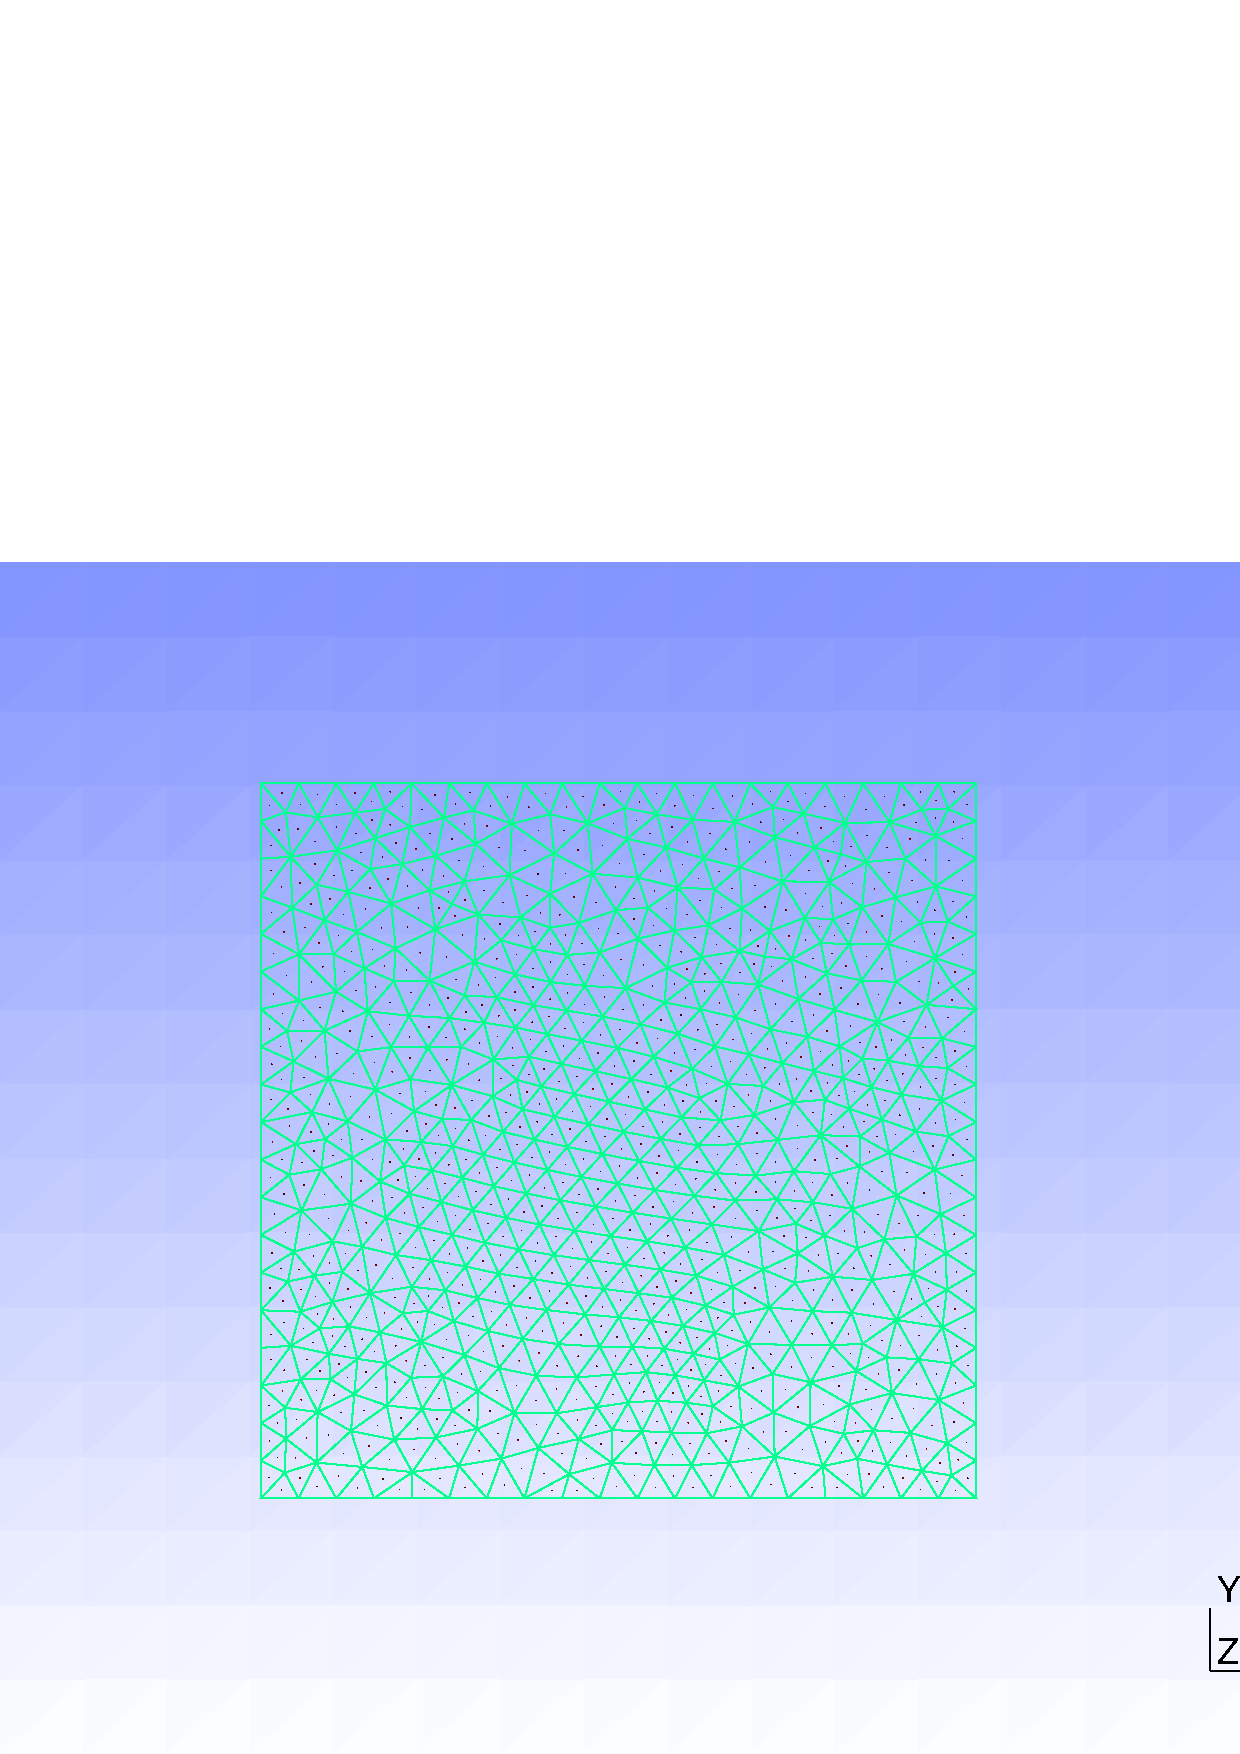
\includegraphics{quad}}
\caption{Quadrilateral with mesh of triangles}
\label{fig:PYCAD 0}
\end{figure}

If you have \gmshextern installed you can run the example and view the
geometry and mesh with:
\begin{verbatim}
run-escript quad.py
gmsh quad.geo
gmsh quad.msh
\end{verbatim}
See Figure~\ref{fig:PYCAD 0} for a result.

In most cases it is best practice to generate the mesh and solve the
mathematical model in two separate scripts. In our example you can read the
\finley mesh into your simulation code\footnote{\gmshextern files can be
directly read using \function{ReadGmsh}, see \Chap{chap:finley}} using
\begin{python}
  from finley import ReadMesh
  mesh=ReadMesh("quad.fly")
\end{python}
Note that the underlying mesh generation software will not accept all
the geometries you can create.  For example, \pycad will happily allow
you to create a 2-D \class{Design} that is a closed loop with some
additional points or lines lying outside of the enclosed area, but
\gmshextern will fail to create a mesh for it.

\section{Holes}
The example included below shows how to use \pycad to create a 2-D mesh
in the shape of a trapezoid with a cut-out area as in Figure~\ref{fig:PYCAD 1}.

\begin{python}
  from esys.pycad import *
  from esys.pycad.gmsh import Design
  from esys.finley import MakeDomain
  
  # A trapezoid
  p0=Point(0.0, 0.0, 0.0)
  p1=Point(1.0, 0.0, 0.0)
  p2=Point(1.0, 0.5, 0.0)
  p3=Point(0.0, 1.0, 0.0)
  l01=Line(p0, p1)
  l12=Line(p1, p2)
  l23=Line(p2, p3)
  l30=Line(p3, p0)
  c=CurveLoop(l01, l12, l23, l30)
  
  # A small triangular cutout
  x0=Point(0.1, 0.1, 0.0)
  x1=Point(0.5, 0.1, 0.0)
  x2=Point(0.5, 0.2, 0.0)
  x01=Line(x0, x1)
  x12=Line(x1, x2)
  x20=Line(x2, x0)
  cutout=CurveLoop(x01, x12, x20)
  
  # Create the surface with cutout
  s=PlaneSurface(c, holes=[cutout])
  
  # Create a Design which can make the mesh
  d=Design(dim=2, element_size=0.05)
  
  # Add the trapezoid with cutout
  d.addItems(s)
  
  # Create the geometry, mesh and Escript domain
  d.setScriptFileName("trapezoid.geo")
  d.setMeshFileName("trapezoid.msh")
  domain=MakeDomain(d)
  # write mesh to a finley file:
  domain.write("trapezoid.fly")
\end{python}
This example is included with the software in \file{trapezoid.py} in the
\ExampleDirectory.

\begin{figure}
\centerline{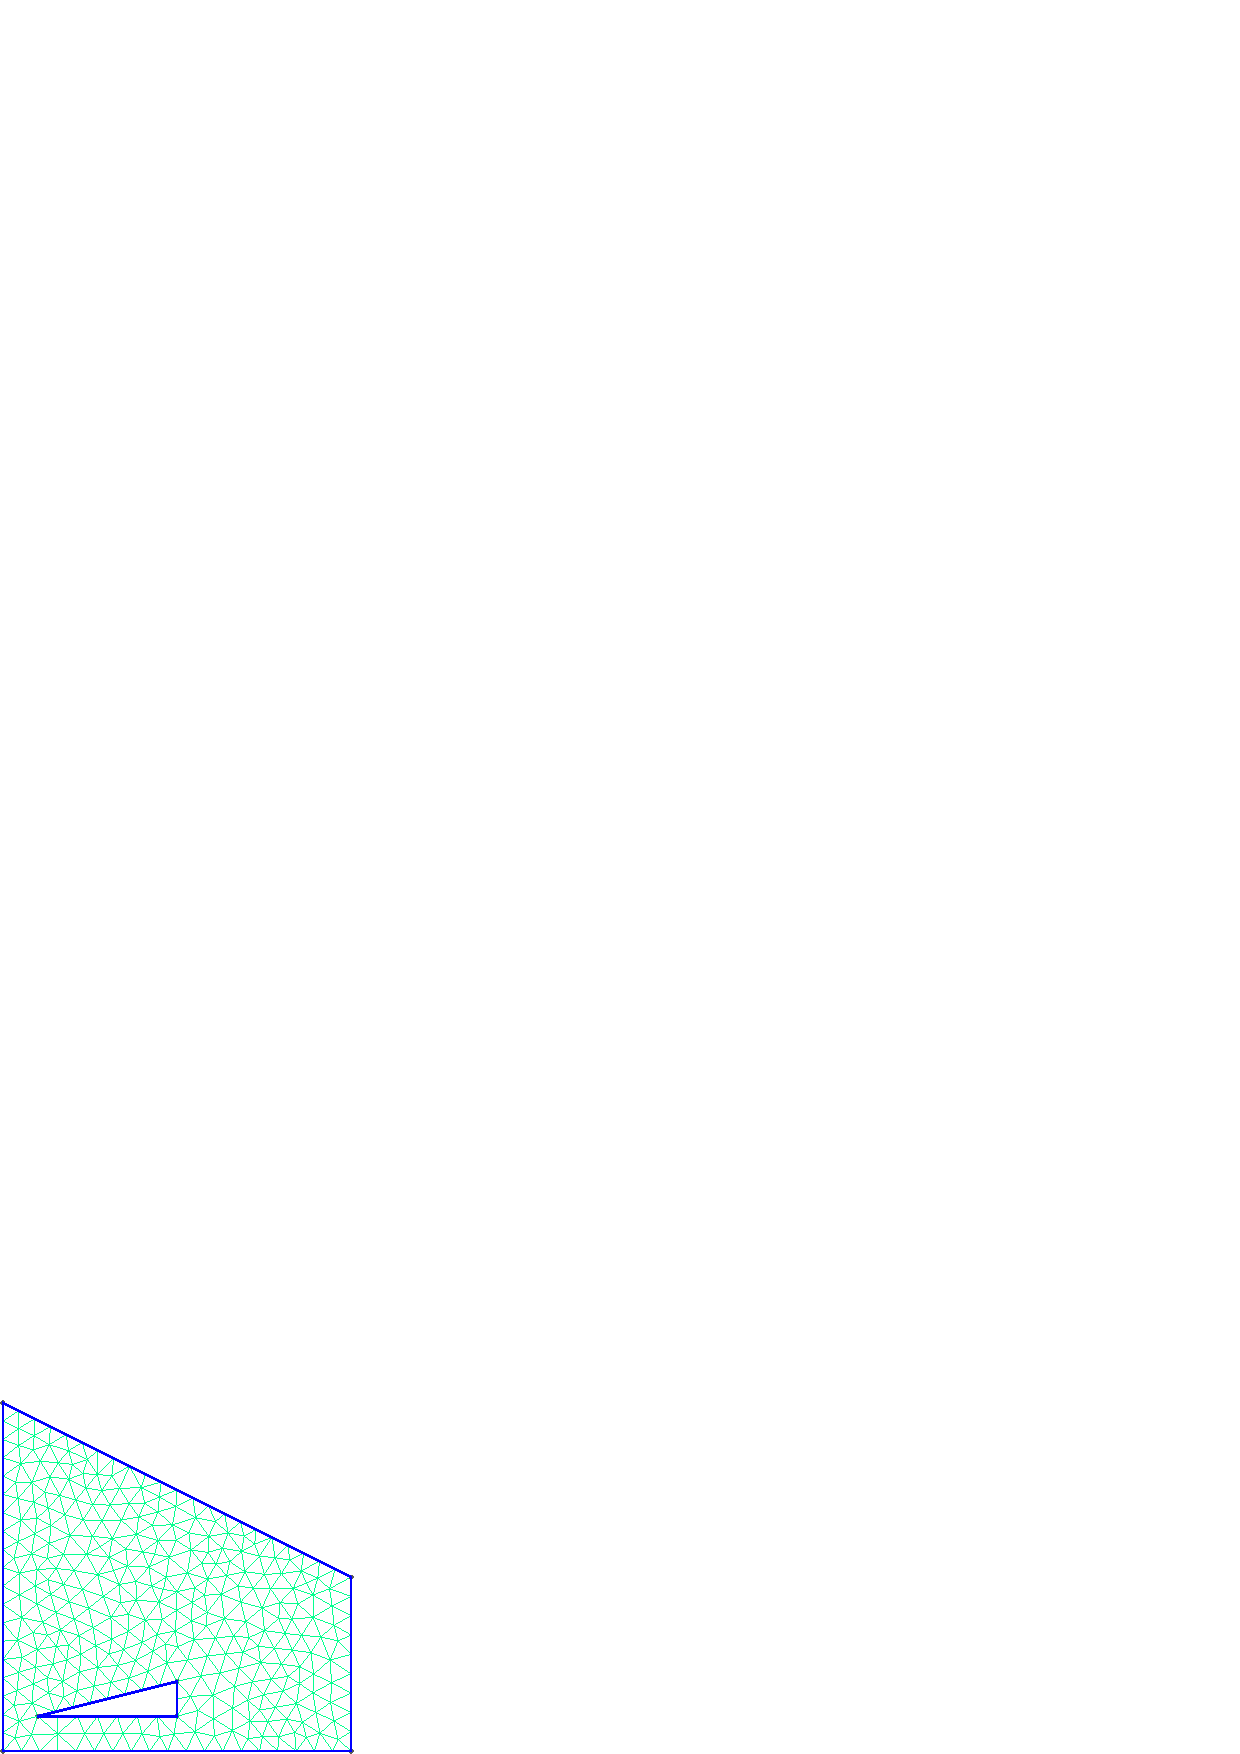
\includegraphics{trapezoid}}
\caption{Trapezoid with triangular hole}
\label{fig:PYCAD 1}
\end{figure}

A \code{CurveLoop} is used to connect several lines into a single curve.
It is used in the example above to create the trapezoidal outline for the grid
and also for the triangular cutout area.
You can define any number of lines when creating a \class{CurveLoop}, but
the end of one line must be identical to the start of the next.

\section{A 3D example}

In this section we discuss the definition of 3D geometries. As an example
consider the unit cube as shown in Figure~\ref{fig:PYCAD 2}.
First we generate the vertices of the cube:
\begin{python}
  from esys.pycad import *
  p0=Point(0.,0.,0.)
  p1=Point(1.,0.,0.)
  p2=Point(0.,1.,0.)
  p3=Point(1.,1.,0.)
  p4=Point(0.,0.,1.)
  p5=Point(1.,0.,1.)
  p6=Point(0.,1.,1.)
  p7=Point(1.,1.,1.)
\end{python}

We connect the points to form the bottom and top surfaces of the cube:
\begin{python}
  l01=Line(p0,p1)
  l13=Line(p1,p3)
  l32=Line(p3,p2)
  l20=Line(p2,p0)
  bottom=PlaneSurface(-CurveLoop(l01,l13,l32,l20))
\end{python}

\begin{figure}
\centerline{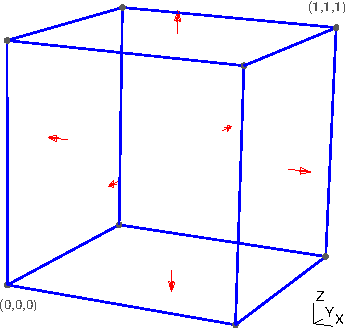
\includegraphics{brick}}
\caption{Three dimensional block}
\label{fig:PYCAD 2}
\end{figure}

Similar to the definition of a \code{CurvedLoop} the orientation of the
surfaces in a \code{SurfaceLoop} is relevant.
In fact, the surface normal direction defined by the right-hand rule needs to
point outwards as indicated by the surface normals in Figure~\ref{fig:PYCAD 2}.
As the \code{bottom} face is directed upwards it is inserted with the minus
sign into the \code{SurfaceLoop} in order to adjust the orientation of the
surface. Similarly we set 
\begin{python}
  l45=Line(p4,p5)
  l57=Line(p5,p7)
  l76=Line(p7,p6)
  l64=Line(p6,p4)
  top=PlaneSurface(CurveLoop(l45,l57,l76,l64))
\end{python}
To form the front face we introduce the two additional lines connecting the
left and right front points of the \code{top} and \code{bottom} face:
\begin{python}
  l15=Line(p1,p5)
  l40=Line(p4,p0)
\end{python}
To form the front face we encounter a problem, the line \code{l45} used
to define the \code{top} face is pointing the wrong direction.
In \pycad you can reverse the direction of an object by changing its sign.
So we write \code{-l45} to indicate that the direction is to be reversed.
With this notation we can write
\begin{python}
  front=PlaneSurface(CurveLoop(l01,l15,-l45,l40))
\end{python}
Keep in mind that if you use \code{Line(p4,p5)} instead of \code{-l45} both
objects are treated as different although connecting the same points with a
straight line in the same direction. The resulting geometry would include an
opening along the \code{p4}--\code{p5} connection.
This will lead to an inconsistent mesh and may result in a failure of the
volumetric mesh generator. Similarly we can define the other sides of the cube:
\begin{python}
  l37=Line(p3,p7)
  l62=Line(p6,p2)
  back=PlaneSurface(CurveLoop(l32,-l62,-l76,-l37))
  left=PlaneSurface(CurveLoop(-l40,-l64,l62,l20))
  right=PlaneSurface(CurveLoop(-l15,l13,l37,-l57))
\end{python}
We can now put the six surfaces together to form a \class{SurfaceLoop}
defining the boundary of the volume of the cube:
\begin{python}
  sl=SurfaceLoop(top,bottom,front,back,left,right)
  v=Volume(sl)
\end{python}
As in the 2D case, the \class{Design} class is used to define the geometry:
\begin{python}
  from esys.pycad.gmsh import Design
  from esys.finley import MakeDomain

  des=Design(dim=3, element_size = 0.1, keep_files=True)
  des.setScriptFileName("brick.geo")
  des.addItems(v, top, bottom, back, front, left, right)

  dom=MakeDomain(des)
  dom.write("brick.fly")
\end{python}
Note that the \finley mesh file \file{brick.fly} will contain the
triangles used to define the surfaces as they are added to the \class{Design}.
The example script of the cube is included with the software in
\file{brick.py} in the \ExampleDirectory.

\section{Alternative File Formats}
\pycad supports other file formats including I-DEAS universal file, VRML,
Nastran and STL. The following example shows how to generate the STL file
\file{brick.stl}:
\begin{python}
  from esys.pycad.gmsh import Design

  des=Design(dim=3, element_size = 0.1, keep_files=True)
  des.addItems(v, top, bottom, back, front, left , right)

  des.setFileFormat(des.STL)
  des.setMeshFileName("brick.stl")
  des.generate()
\end{python}
The example script of the cube is included with the software in
\file{brick_stl.py} in the \ExampleDirectory.

\section{Element Sizes}
The element size used globally is defined by the \code{element_size} argument
of the \class{Design}. The mesh generator will try to use this mesh size
everywhere in the geometry. In some cases it can be desirable to use a finer
mesh locally. A local refinement can be defined at each \class{Point}:
\begin{python}
  p0=Point(0., 0., 0., local_scale=0.01)
\end{python}
Here the mesh generator will create a mesh with an element size which is by
the factor \code{0.01} times smaller than the global mesh size
\code{element_size=0.3}, see Figure~\ref{fig:PYCAD 5}.
The point where a refinement is defined must be a point on a curve used to
define the geometry.

\begin{figure}
\centerline{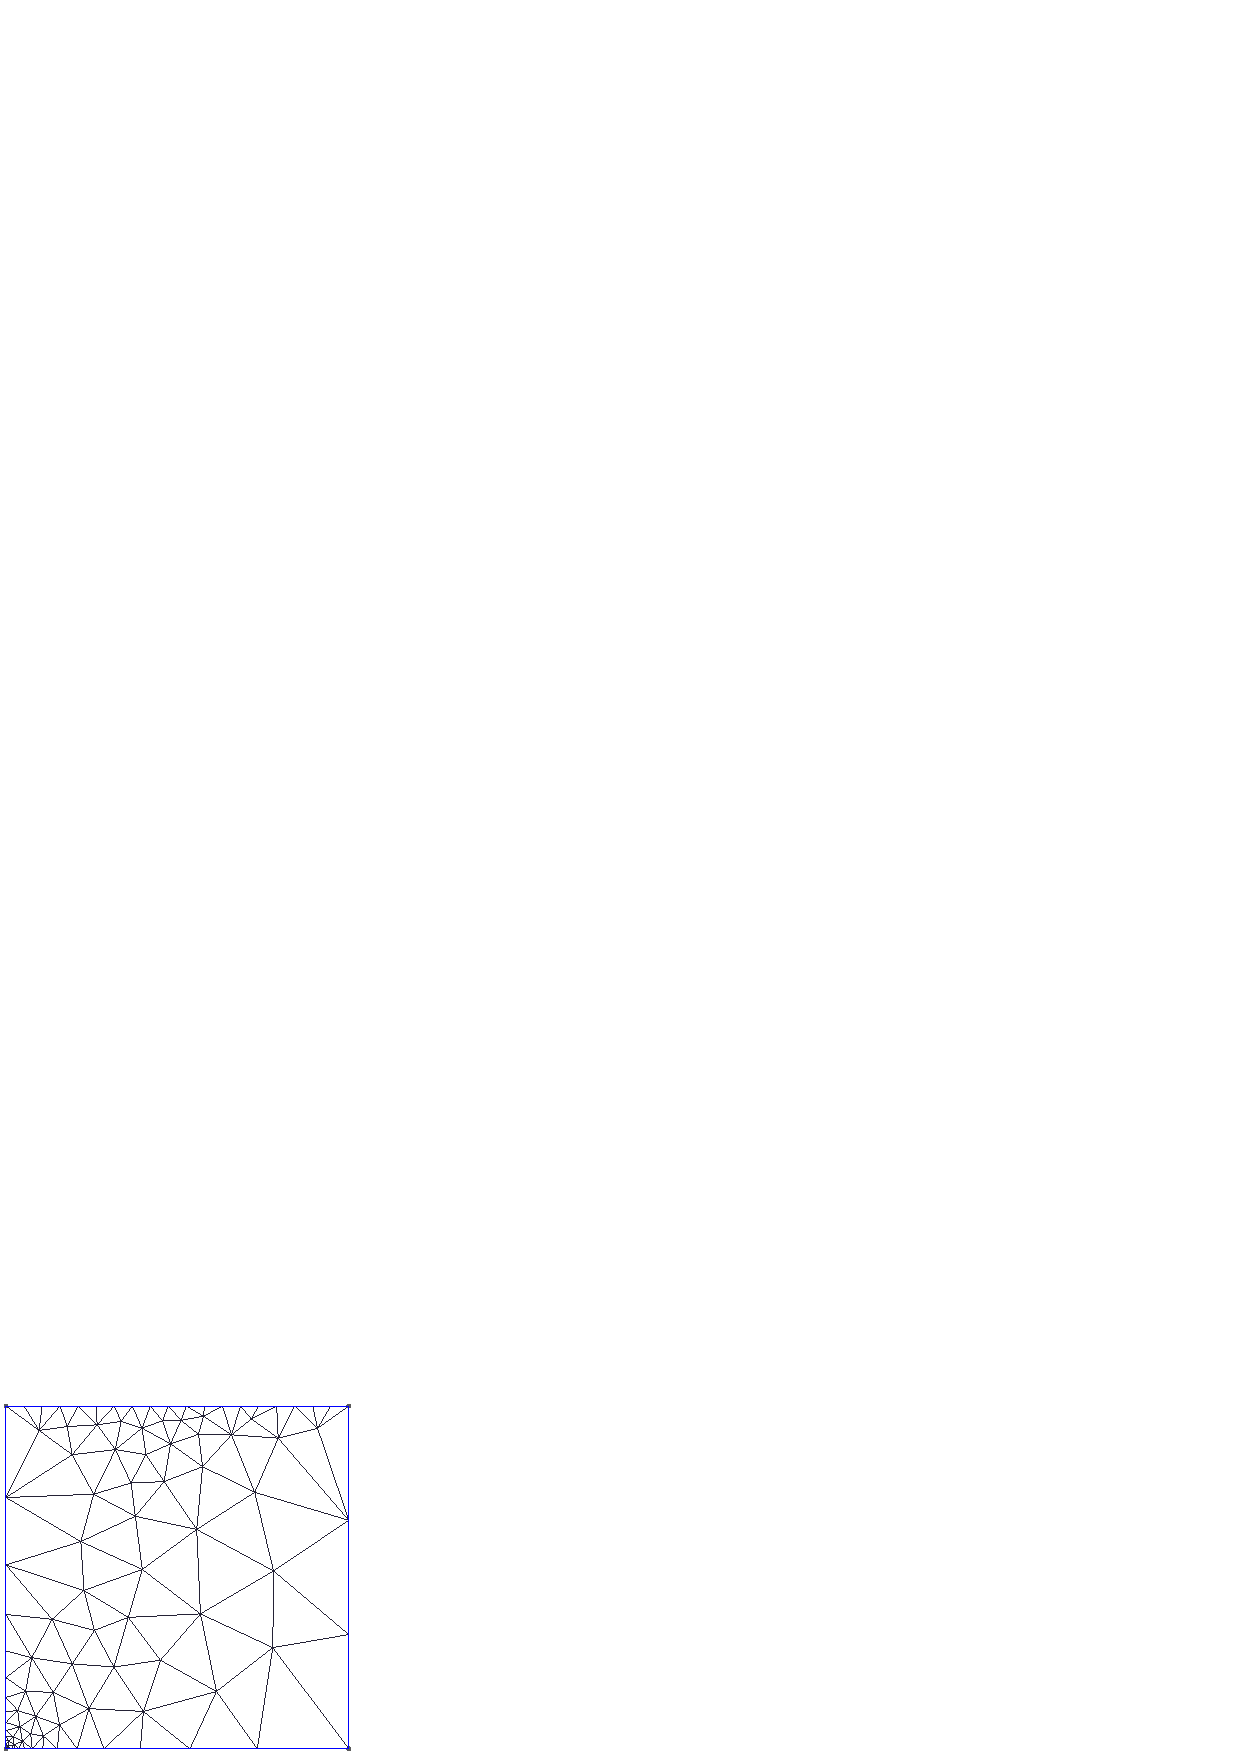
\includegraphics{refine}}
\caption{Local refinement at the origin by \var{local_scale=0.01}
with \var{element_size=0.3} and number of elements on the top set to 10}
\label{fig:PYCAD 5}
\end{figure}

Alternatively, one can define a mesh size along a curve by defining the number
of elements to be used to subdivide the curve. For instance, to use $20$
elements on line \code{l23}:
\begin{python}
  l23=Line(p2, p3)
  l23.setElementDistribution(20)
\end{python}
Setting the number of elements on a curve overwrites the global mesh size
\code{element_size}. The result is shown in Figure~\ref{fig:PYCAD 5}.

\section{\pycad Classes}
%\declaremodule{extension}{esys.pycad}
%\modulesynopsis{Python geometry description and meshing interface}

\subsection{Primitives}
Some of the most commonly-used objects in \pycad are listed here.
For a more complete list see the full API documentation.

\begin{classdesc}{Point}{x=0.,y=0.,z=0.\optional{,local_scale=1.}}
creates a point at the given coordinates with local characteristic length \var{local_scale}
\end{classdesc}

\begin{classdesc}{CurveLoop}{list}
creates a closed curve from a \code{list} of
\class{Line}, \class{Arc}, \class{Spline}, \class{BSpline},
\class{BezierSpline} objects.
\end{classdesc}

\begin{classdesc}{SurfaceLoop}{list}
creates a loop of \class{PlaneSurface} or \class{RuledSurface}, which defines
the shell of a volume.
\end{classdesc}

\subsubsection{Lines}
\begin{classdesc}{Line}{point1, point2}
creates a line between two points.
\end{classdesc}

\begin{methoddesc}[Line]{setElementDistribution}{n\optional{,progression=1\optional{,createBump=\False}}}
defines the number of elements on the line. If set, it overwrites the local
length setting which would be applied.
The progression factor \var{progression} defines the change of element size
between neighboured elements. If \var{createBump} is set progression is
applied towards the centre of the line.
\end{methoddesc}

\begin{methoddesc}[Line]{resetElementDistribution}{}
removes a previously set element distribution from the line.
\end{methoddesc}
\begin{methoddesc}[Line]{getElementDistribution}{}
returns the element distribution as a tuple of number of elements, progression
factor and bump flag. If no element distribution is set None is returned.
\end{methoddesc}

\subsubsection{Splines}
\begin{classdesc}{Spline}{point0, point1, ...}
A spline curve defined by a list of points \var{point0}, \var{point1}, \ldots
\end{classdesc}

\begin{methoddesc}[Spline]{setElementDistribution}{n\optional{,progression=1\optional{,createBump=\False}}}
defines the number of elements on the spline. If set, it overwrites the local
length setting which would be applied.
The progression factor \var{progression} defines the change of element size
between neighboured elements. If \var{createBump} is set progression is
applied towards the centre of the spline.
\end{methoddesc}

\begin{methoddesc}[Spline]{resetElementDistribution}{}
removes a previously set element distribution from the spline.
\end{methoddesc}

\begin{methoddesc}[Spline]{getElementDistribution}{}
returns the element distribution as a tuple of number of elements, progression
factor and bump flag. If no element distribution is set None is returned.
\end{methoddesc}

\subsubsection{BSplines}
\begin{classdesc}{BSpline}{point0, point1, ...}
A B-spline curve defined by a list of points \var{point0}, \var{point1}, \ldots
\end{classdesc}

\begin{methoddesc}[BSpline]{setElementDistribution}{n\optional{,progression=1\optional{,createBump=\False}}}
defines the number of elements on the curve. If set, it overwrites the local
length setting which would be applied.
The progression factor \var{progression} defines the change of element size
between neighboured elements. If \var{createBump} is set progression is
applied towards the centre of the curve.
\end{methoddesc}

\begin{methoddesc}[BSpline]{resetElementDistribution}{}
removes a previously set element distribution from the curve.
\end{methoddesc}

\begin{methoddesc}[BSpline]{getElementDistribution}{}
returns the element distribution as a tuple of number of elements, progression
factor and bump flag. If no element distribution is set None is returned.
\end{methoddesc}

\subsubsection{Bezier Curves}
\begin{classdesc}{BezierCurve}{point0, point1, ...}
A Bezier spline curve defined by a list of points \var{point0}, \var{point1}, \ldots
\end{classdesc}

\begin{methoddesc}[BezierCurve]{setElementDistribution}{n\optional{,progression=1\optional{,createBump=\False}}}
defines the number of elements on the curve. If set, it overwrites the local
length setting which would be applied.
The progression factor \var{progression} defines the change of element size
between neighboured elements. If \var{createBump} is set progression is
applied towards the centre of the curve.
\end{methoddesc}

\begin{methoddesc}[BezierCurve]{resetElementDistribution}{}
removes a previously set element distribution from the curve.
\end{methoddesc}

\begin{methoddesc}[BezierCurve]{getElementDistribution}{}
returns the element distribution as a tuple of number of elements, progression
factor and bump flag. If no element distribution is set None is returned.
\end{methoddesc}

\subsubsection{Arcs}
\begin{classdesc}{Arc}{centre_point, start_point, end_point}
creates an arc by specifying a centre for a circle and start and end points.
An arc may subtend an angle of at most $\pi$ radians.
\end{classdesc}

\begin{methoddesc}[Arc]{setElementDistribution}{n\optional{,progression=1\optional{,createBump=\False}}}
defines the number of elements on the arc. If set, it overwrites the local
length setting which would be applied.
The progression factor \var{progression} defines the change of element size
between neighboured elements. If \var{createBump} is set progression is
applied towards the centre of the arc.
\end{methoddesc}

\begin{methoddesc}[Arc]{resetElementDistribution}{}
removes a previously set element distribution from the arc.
\end{methoddesc}

\begin{methoddesc}[Arc]{getElementDistribution}{}
returns the element distribution as a tuple of number of elements, progression
factor and bump flag. If no element distribution is set None is returned.
\end{methoddesc}

\subsubsection{Plane surfaces}
\begin{classdesc}{PlaneSurface}{loop, \optional{holes=[list]}}
creates a plane surface from a \class{CurveLoop}, which may have one or more
holes described by a \var{list} of \class{CurveLoop} objects.
\end{classdesc}

\begin{methoddesc}[PlaneSurface]{setElementDistribution}{n\optional{,progression=1\optional{,createBump=\False}}}
defines the number of elements on all lines.
\end{methoddesc}

\begin{methoddesc}[PlaneSurface]{setRecombination}{\optional{max_deviation=45 * \var{DEG} }}
the mesh generator will try to recombine triangular elements into
quadrilateral elements. \var{max_deviation} (in radians) defines the
maximum deviation of any angle in the quadrilaterals from the right angle.
Set \var{max_deviation}=\var{None} to remove recombination.
\end{methoddesc}

\begin{methoddesc}[PlaneSurface]{setTransfiniteMeshing}{\optional{orientation="Left"}}
applies 2D transfinite meshing to the surface.
\var{orientation} defines the orientation of triangles. Allowed values
are \var{``Left''}, \var{``Right''} and \var{``Alternate''}.
The boundary of the surface must be defined by three or four lines and an
element distribution must be defined on all faces where opposite
faces use the same element distribution. No holes must be present.
\end{methoddesc}

\subsubsection{Ruled Surfaces}
\begin{classdesc}{RuledSurface}{list}
creates a surface that can be interpolated using transfinite interpolation.
\var{list} gives a list of three or four lines defining the boundary of the
surface.
\end{classdesc}

\begin{methoddesc}[RuledSurface]{setRecombination}{\optional{max_deviation=45 * \var{DEG} }}
the mesh generator will try to recombine triangular elements into
quadrilateral elements. \var{max_deviation} (in radians) defines the
maximum deviation of any angle in the quadrilaterals from the right angle.
Set \var{max_deviation}=\var{None} to remove recombination.
\end{methoddesc}

\begin{methoddesc}[RuledSurface]{setTransfiniteMeshing}{\optional{orientation="Left"}}
applies 2D transfinite meshing to the surface.
\var{orientation} defines the orientation of triangles. Allowed values
are \var{``Left''}, \var{``Right''} and \var{``Alternate''}.
The boundary of the surface must be defined by three or four lines and an
element distribution must be defined on all faces where opposite
faces use the same element distribution. No holes must be present.
\end{methoddesc}

\begin{methoddesc}[RuledSurface]{setElementDistribution}{n\optional{,progression=1\optional{,createBump=\False}}}
defines the number of elements on all lines.
\end{methoddesc}

\subsubsection{Volumes}
\begin{classdesc}{Volume}{loop, \optional{holes=[list]}}
creates a volume given a \class{SurfaceLoop}, which may have one or more holes
define by the list of \class{SurfaceLoop}.
\end{classdesc}

\begin{methoddesc}[Volume]{setElementDistribution}{n\optional{,progression=1\optional{,createBump=\False}}}
defines the number of elements on all lines.
\end{methoddesc}

\begin{methoddesc}[Volume]{setRecombination}{\optional{max_deviation=45 * \var{DEG} }}
the mesh generator will try to recombine triangular elements into
quadrilateral elements. These meshes are then used to generate the volume mesh
if possible.
Together with transfinite meshing one can construct rectangular meshes.
\var{max_deviation} (in radians) defines the maximum deviation of any angle in
the quadrilaterals from the right angle.
Set \var{max_deviation}=\var{None} to remove recombination.
\end{methoddesc}

\begin{methoddesc}[Volume]{setTransfiniteMeshing}{\optional{orientation="Left"}}
applies transfinite meshing to the volume and all surfaces (if
\var{orientation} is not equal to \var{None}).
\var{orientation} defines the orientation of triangles. Allowed values
are \var{``Left''}, \var{``Right''} and \var{``Alternate''}.
The boundary of the surface must be defined by three or four lines and an
element distribution must be defined on all faces where opposite
faces use the same element distribution.
If \var{orientation} is equal to \var{None} transfinite meshing is not
switched on for the surfaces but needs to be set by the user.
No holes must be present.
\textbf{Warning: The functionality of transfinite meshing without
recombination is not entirely clear in \gmshextern.
So please apply this method with care.}
\end{methoddesc}

%============================================================================
\subsection{Transformations}

Sometimes it is convenient to create an object and then make copies at
different orientations or in different sizes. This can be achieved by
applying transformations which are used to move geometrical objects in the
3-dimensional space and to resize them.

\begin{classdesc}{Translation}{\optional{b=[0,0,0]}}
defines a translation $x \to x+b$. \var{b} can be any object that can be
converted into a \numpy object of shape $(3,)$.
\end{classdesc}

\begin{classdesc}{Rotation}{\optional{axis=[1,1,1], \optional{ point = [0,0,0], \optional{angle=0*RAD} } } }
defines a rotation by \var{angle} around axis through point \var{point} and direction \var{axis}.
\var{axis} and \var{point} can be any object that can be converted into a
\numpy object of shape $(3,)$.
\var{axis} does not have to be normalised but must have positive length.
The right-hand rule~\cite{RIGHTHANDRULE} applies.
\end{classdesc}

\begin{classdesc}{Dilation}{\optional{factor=1., \optional{centre=[0,0,0]}}}
defines a dilation by the expansion/contraction \var{factor} with
\var{centre} as the dilation centre.
\var{centre} can be any object that can be converted into a \numpy object of
shape $(3,)$.
\end{classdesc}

\begin{classdesc}{Reflection}{\optional{normal=[1,1,1], \optional{offset=0}}}
defines a reflection on a plane defined in normal form $n^t x = d$
where $n$ is the surface normal \var{normal} and $d$ is the plane \var{offset}.
\var{normal} can be any object that can be converted into a \numpy object of
shape $(3,)$.
\var{normal} does not have to be normalised but must have positive length.
\end{classdesc}

\begin{datadesc}{DEG}
a constant to convert from degrees to an internal angle representation in
radians. For instance use \code{90*DEG} for $90$ degrees.
\end{datadesc}

\subsection{Properties}
If you are building a larger geometry you may find it convenient to
create it in smaller pieces and then assemble them.
Property Sets make this easy, and they allow you to name the smaller
pieces for convenience.

Property Sets are used to bundle a set of geometrical objects in a
group. The group is identified by a name. Typically a Property Set
is used to mark subregions which share the same material properties or
to mark portions of the boundary. For efficiency, the \Design class
assigns an integer to each of its Property Sets, a so-called tag\index{tag}.
The appropriate tag is attached to the elements at generation time.

See the file \code{pycad/examples/quad.py} for an example using a {\it PropertySet}.

\begin{classdesc}{PropertySet}{name,*items}
defines a group geometrical objects which can be accessed through a \var{name}
The objects in the tuple \var{items} mast all be \ManifoldOneD, \ManifoldTwoD or \ManifoldThreeD objects.
\end{classdesc}

\begin{methoddesc}[PropertySet]{getManifoldClass}{}
returns the manifold class \ManifoldOneD, \ManifoldTwoD or \ManifoldThreeD
expected from the items in the property set.
\end{methoddesc}

\begin{methoddesc}[PropertySet]{getDim}{}
returns the spatial dimension of the items in the property set.
\end{methoddesc}

\begin{methoddesc}[PropertySet]{getName}{}
returns the name of the set
\end{methoddesc}

\begin{methoddesc}[PropertySet]{setName}{name}
sets the name. This name should be unique within a \Design.
\end{methoddesc}

\begin{methoddesc}[PropertySet]{addItem}{*items}
adds a tuple of items. They need to be objects of class \ManifoldOneD,
\ManifoldTwoD or \ManifoldThreeD.
\end{methoddesc}

\begin{methoddesc}[PropertySet]{getItems}{}
returns the list of items
\end{methoddesc}

\begin{methoddesc}[PropertySet]{clearItems}{}
clears the list of items
\end{methoddesc}

\begin{methoddesc}[PropertySet]{getTag}{}
returns the tag used for this property set
\end{methoddesc}

\section{Interface to the mesh generation software}
%\declaremodule{extension}{esys.pycad.gmsh}
%\modulesynopsis{Python geometry description and meshing interface}

The class and methods described here provide an interface to the mesh
generation software, which is currently \gmshextern. This interface could be
adopted to \emph{triangle} or another mesh generation package if this is
deemed to be desirable in the future.

\begin{classdesc}{Design}{
\optional{dim=3, \optional{element_size=1., \optional{order=1, \optional{keep_files=False}}}}}
describes the geometry defined by primitives to be meshed.
\var{dim} specifies the spatial dimension, while \var{element_size} defines
the global element size which is multiplied by the local scale to set the
element size at each \Point.
The argument \var{order} defines the element order to be used.
If \var{keep_files} is set to \True temporary files are kept, otherwise they
are removed when the instance of the class is deleted.
\end{classdesc}

\begin{memberdesc}[Design]{GMSH}
gmsh file format~\cite{GMSH}
\end{memberdesc}

\begin{memberdesc}[Design]{IDEAS}
I-DEAS universal file format~\cite{IDEAS}
\end{memberdesc}

\begin{memberdesc}[Design]{VRML}
VRML file format, \cite{VRML}
\end{memberdesc}

\begin{memberdesc}[Design]{STL}
STL file format~\cite{STL}
\end{memberdesc}

\begin{memberdesc}[Design]{NASTRAN}
NASTRAN bulk data format~\cite{NASTRAN}
\end{memberdesc}

\begin{memberdesc}[Design]{MEDIT}
Medit file format~\cite{MEDIT}
\end{memberdesc}

\begin{memberdesc}[Design]{CGNS}
CGNS file format~\cite{CGNS}
\end{memberdesc}

\begin{memberdesc}[Design]{PLOT3D}
Plot3D file format~\cite{PLOT3D}
\end{memberdesc}

\begin{memberdesc}[Design]{DIFFPACK}
Diffpack 3D file format~\cite{DIFFPACK}
\end{memberdesc}

\begin{memberdesc}[Design]{DELAUNAY}
the Delaunay triangulator, see \gmshextern and \cite{TETGEN}
\end{memberdesc}

\begin{memberdesc}[Design]{MESHADAPT}
the gmsh triangulator, see \gmshextern
\end{memberdesc}

\begin{memberdesc}[Design]{FRONTAL}
the NETGEN~\cite{NETGEN} triangulator
\end{memberdesc}

\begin{methoddesc}[Design]{generate}{}
generates the mesh file. The data are written to the file \var{Design.getMeshFileName}.
\end{methoddesc}

\begin{methoddesc}[Design]{setDim}{\optional{dim=3}}
sets the spatial dimension which needs to be $1$, $2$ or $3$.
\end{methoddesc}

\begin{methoddesc}[Design]{getDim}{}
returns the spatial dimension.
\end{methoddesc}

\begin{methoddesc}[Design]{setElementOrder}{\optional{order=1}}
sets the element order which needs to be $1$ or $2$.
\end{methoddesc}

\begin{methoddesc}[Design]{getElementOrder}{}
returns the element order.
\end{methoddesc}

\begin{methoddesc}[Design]{setElementSize}{\optional{element_size=1}}
sets the global element size. The local element size at a point is defined as
the global element size multiplied by the local scale.
The element size must be positive.
\end{methoddesc}

\begin{methoddesc}[Design]{getElementSize}{}
returns the global element size.
\end{methoddesc}

\begin{methoddesc}[Design]{setKeepFilesOn}{}
work files are kept at the end of the generation.
\end{methoddesc}

\begin{methoddesc}[Design]{setKeepFilesOff}{}
work files are deleted at the end of the generation.
\end{methoddesc}

\begin{methoddesc}[Design]{keepFiles}{}
returns \True if work files are kept, \False otherwise.
\end{methoddesc}

\begin{methoddesc}[Design]{setScriptFileName}{\optional{name=None}}
sets the file name for the gmsh input script.
If no name is given a name with extension "geo" is generated.
\end{methoddesc}

\begin{methoddesc}[Design]{getScriptFileName}{}
returns the name of the file for the gmsh script.
\end{methoddesc}

\begin{methoddesc}[Design]{setMeshFileName}{\optional{name=None}}
sets the name for the mesh file. If no name is given a name is generated.
The format is set by \\\var{Design.setFileFormat}.
\end{methoddesc}

\begin{methoddesc}[Design]{getMeshFileName}{}
returns the name of the mesh file.
\end{methoddesc}

\begin{methoddesc}[Design]{addItems}{*items}
adds the tuple of \var{items}. An item can be any primitive or a
\class{PropertySet}.
\warning{If a \PropertySet is added which includes an object that is not
part of a \PropertySet, it may not be considered in the meshing.}
\end{methoddesc}

\begin{methoddesc}[Design]{getItems}{}
returns a list of the items.
\end{methoddesc}

\begin{methoddesc}[Design]{clearItems}{}
resets the items in this design.
\end{methoddesc}

\begin{methoddesc}[Design]{getMeshHandler}{}
returns a handle to the mesh.
Calling this method generates the mesh from the geometry and returns a
mechanism to access the mesh data. In the current implementation this
method returns a file name for a file containing the mesh data.
\end{methoddesc}

\begin{methoddesc}[Design]{getScriptString}{}
returns the gmsh script to generate the mesh as a string.
\end{methoddesc}

\begin{methoddesc}[Design]{getCommandString}{}
returns the gmsh command used to generate the mesh as a string.
\end{methoddesc}

\begin{methoddesc}[Design]{setOptions}{
\optional{algorithm=None
\optional{, optimize_quality=\True
\optional{, smoothing=1
\optional{, curvature_based_element_size=\False
\optional{, algorithm2D=None
\optional{, algorithm3D=None
\optional{, generate_hexahedra=False
\optional{, random_factor=None}}}}}}}}}
sets options for the mesh generator.
Both \var{algorithm} and \var{algorithm2D} set the 2D meshing algorithm to be
used. If both parameters are given, they must be equal.
The algorithm needs to be \var{Design.DELAUNAY}, \var{Design.FRONTAL},
or \var{Design.MESHADAPT}. By default \var{Design.MESHADAPT} is used.
\var{algorithm3D} sets the 3D  meshing algorithm to be used.
The algorithm needs to be \var{Design.DELAUNAY} or \var{Design.FRONTAL}.
By default \var{Design.FRONTAL} is used.
\var{optimize_quality}=\True invokes an optimization of the mesh quality.
\var{smoothing} sets the number of smoothing steps to be applied to the mesh.
\var{curvature_based_element_size}=\True switches on curvature based
definition of element size.
\var{generate_hexahedra}=\True switches on the usage of quadrilateral or
hexahedral elements.
\var{random_factor} a positive amount used in the 2D meshing algorithm.
\end{methoddesc}

\begin{methoddesc}[Design]{getTagMap}{}
returns a \class{TagMap} to map the \class{PropertySet} names to tag numbers
generated by gmsh.
\end{methoddesc}

\begin{methoddesc}[Design]{setFileFormat}{\optional{format=\var{Design.GMSH}}}
sets the file format. \var{format} must be one of the values:\\
\var{Design.GMSH}\\
\var{Design.IDEAS}\\
\var{Design.VRML}\\
\var{Design.STL}\\
\var{Design.NASTRAN}\\
\var{Design.MEDIT}\\
\var{Design.CGNS}\\
\var{Design.PLOT3D}\\
\var{Design.DIFFPACK}.
\end{methoddesc}

\begin{methoddesc}[Design]{getFileFormat}{}
returns the file format.
\end{methoddesc}

